\section{Materiales y métodos}

Con el objetivo de estudiar el efecto Skin sobre un material conductor, se utilizó el dispositivo experimental presentado en la \autoref{fig:disp exp}, el cual consistía en un transformador conmformado por una bobina primaria ($P$) de 1600 vueltas e inductancia de \SI{52(1)}{\milli\henry} y una bobina secundaria ($S$) de 3200 vueltas e inductancia de \SI{207(1)}{\milli\henry}, ambas incrustadas en un núcleo de hierro. La bobina primaria se encontraba conectada a un generador de señales sinusoidales y a una resistencia $R$ de \SI{40,1(2,0)}{\ohm}, de manera de obtener la corriente del circuito al medir la diferencia de potencial $V_P$ entre sus extremos utilizando un osciloscopio, mientras que sobre la bobina secundaria se medía directamente la dferencia de potencial $V_S$.
\begin{figure}[H]
    \centering
    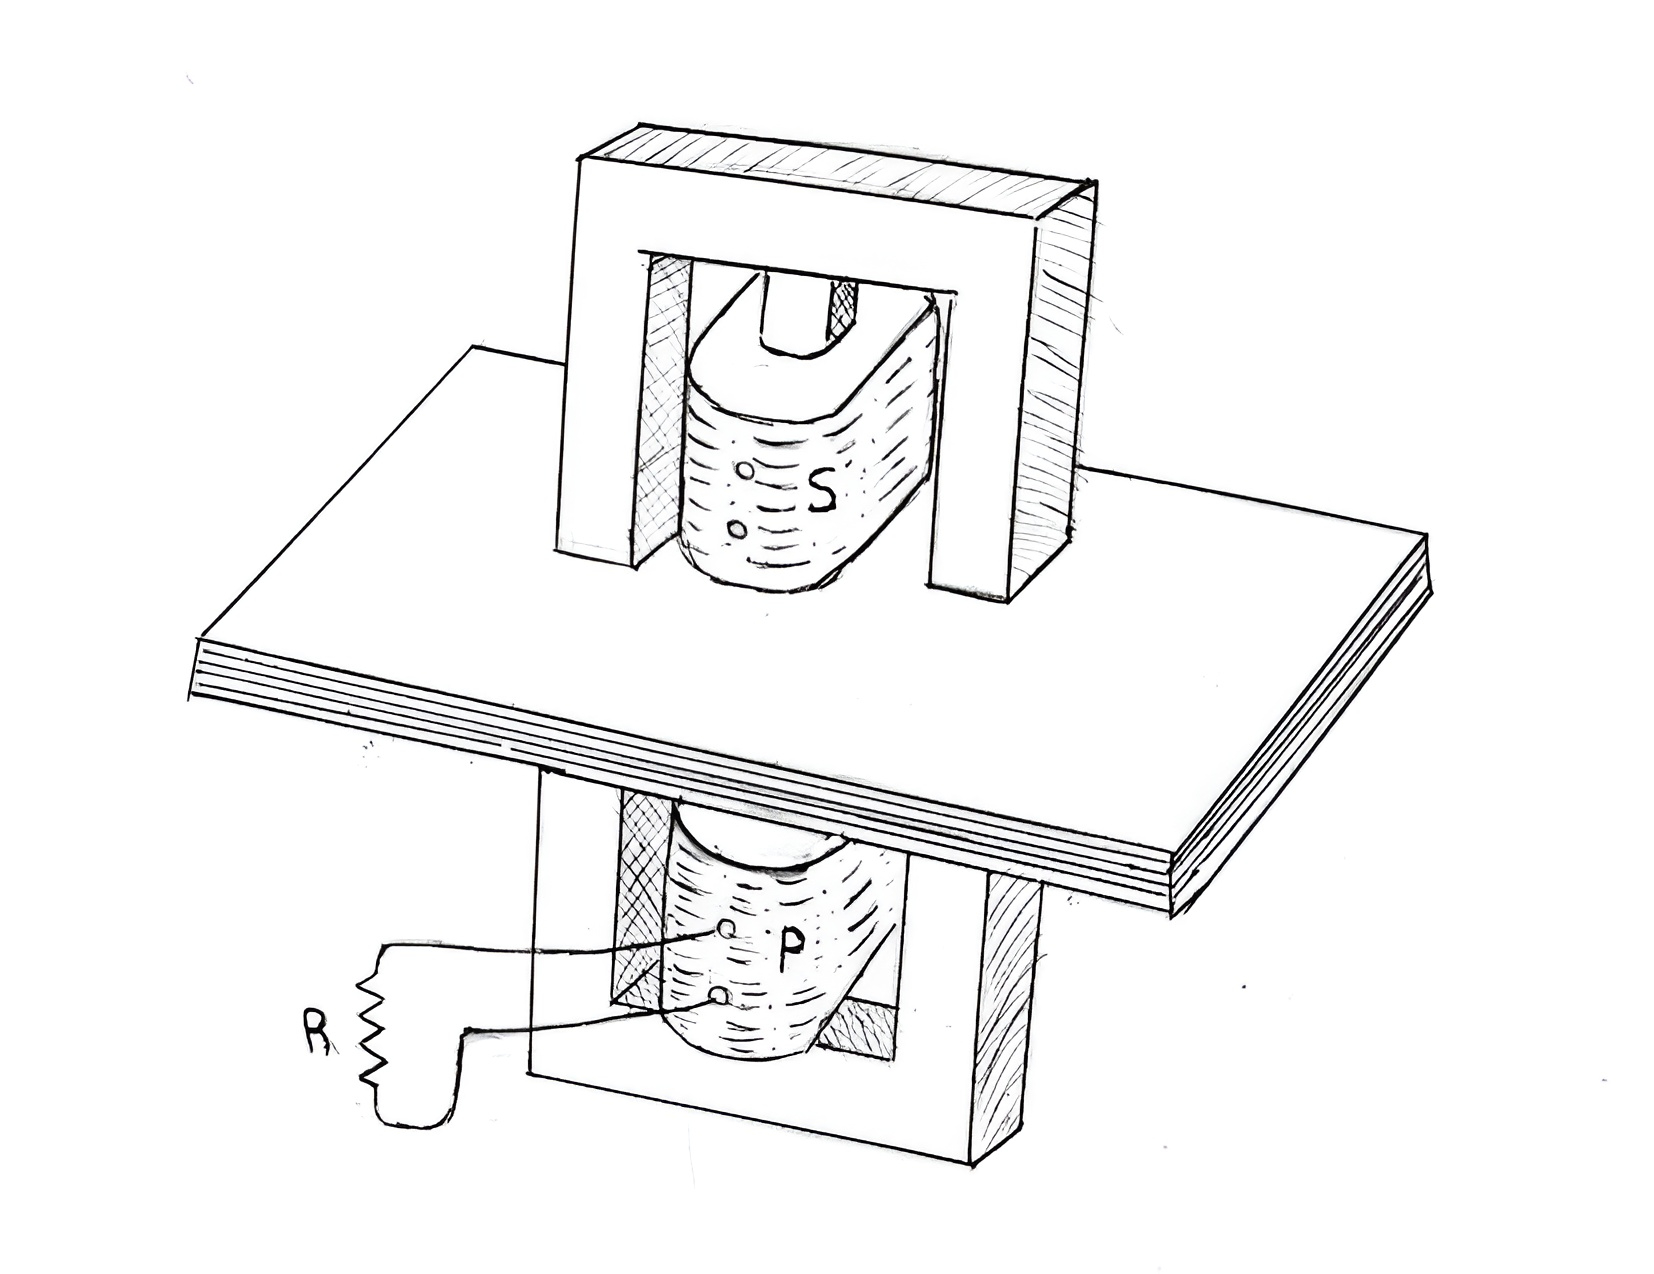
\includegraphics[width=0.5\textwidth]{Figuras 3/disp_exp.jpg}
    \caption{Esquema del dispositivo experimental utilizado para estudiar el efecto Skin. Entre la bobina primaria $P$ y la bobina secundaria $S$ se colocan placas de aluminio. Conectada a la bobina primaria se encuentra una resistencia $R$, sobre la cual se mide la diferencia de potencial $V_P$, mientras que sobre la bobina secundaria se mide la diferencia de potencial $V_S$, utilizando un osciloscopio.}
    \label{fig:disp exp}
\end{figure}

Entre ambas bobinas se colocaron diversas placas de aluminio, las cuales variaban según el experimento realizado: espesor fijo o frecuencia fija. Para el experimento a espesor fijo, se colocó una única placa de \SI{1.56(1)}{\milli\meter} de espesor, y se variaron las frecuencias de la señal entre [20, 820] \si{\hertz}. Para el experimento a frecuencia fija, se utilizó una señal de \SI{50,0(2,5)}{\hertz} y se varió el espesor del material colocando sucesivamente placas una encima de la otra. En ambos experimentos, se midió la caida de potencial sobre la bobina secundaria y la resistencia conectada a la bobina primaria, junto al desfasaje entre ambas señales a partir de la relación $\phi = 2\pi f \Delta t$.

Para la serie de datos con espesor fijo, se graficó el desfasaje $\phi$ y el cociente entre el módulo de la función de transferencia $|H| = \frac{V_S}{V_P}$ y la frecuencia angular $\omega = 2\pi f$, en función de $\sqrt{\omega}$. En busca de obtener la conductvidad $\sigma$, se realizaron dos ajustes, según la expresión para el módulo dada por
\begin{equation}
    \frac{|H|}{\omega} = A \psi(z, \omega)
    \label{eq: modulo-z fijo}
\end{equation}

donde $\psi(z, \omega)$ es la función de onda dada por la ecuación \eqref{eq: psi(z)} y A es un parámetro libre, y utilizando la expresión para la fase 

\begin{equation}
 \phi = \frac{1}{\delta} z + a
 \label{eq: fase-z fijo}
\end{equation} 

con $a$ libre.

Para la serie de datos con frecuencia fija, se graficó el desfasaje $\phi$ y el módulo $|H|$, en función del espesor $z$. Para obtener $\delta$, se realizaron dos ajustes, utilizando la ecuación

\begin{equation}
    |H| = B \psi(z, \omega)
    \label{eq: modulo-f fijo}
\end{equation}
donde B es un parámetro libre, y de la expresión para la fase dada por
\begin{equation}
    \phi = \frac{1}{\delta} z + b
    \label{eq: fase-f fijo}
\end{equation}
con $b$ libre.